\chapter{Infrastructure}\label{chap:infrastructure}

The purpose of infrastructure is to develop a set of tools to assist
in the creation of the product by automating a specific set of actions
or behaviour. In software projects, these tools broadly fall into one
of three categories: build automation, testing automation, and task
automation. In all cases, their primary purposes is to save developer
time and reduce the risk of human error by automating repeatable
tasks. The development of tooling was assigned a high priority
throughout the project due to its mitigating effects on the risks of
technical complexity and deployment complexity. Additionally, it is
often possible to repurpose tools for multiple projects, which helps
satisfy the high project objective of producing something of real
world value for future work.

\section{Build automation}\label{sec:build-automation}

The building and compilation stage for pip-db requires the execution
of many steps, the most notable of which are:

\begin{itemize}
\item \textbf{Clojure compilation} The web server is written in
  Clojure LISP, which is a compiled language that must be compiled
  into Java bytecode for execution on the Java Virtual Machine (see
  Section~\ref{sec:programming-language-choice}).
\item \textbf{JavaScript minification} Client-side scripts are
  pre-processed using a minifier, which is program that reduces the
  size of a source code by removing all unnecessary characters, and
  further reduces the size of the source code through semantic
  evaluation of the code in order to produce shorter variable names
  and generate compacted source code. The purpose of generating a
  compacted file is to reduce the bandwidth required to transmit it to
  the client, resulting in faster page loading times.
\item \textbf{Stylesheet pre-processing} Client-side stylesheets are
  written in Less CSS, which is a language which compiles to CSS and
  offers extensions to the CSS specification, such as variables and
  control flow. Additionally, compiled CSS stylesheets are minified to
  reduce their size.
\item \textbf{Documentation rendering} User documentation is compiled
  from intermediate forms (\LaTeX, Markdown) into publishable formats
  (pdf, HTML).
\item \textbf{Binary installation} Executable scripts and applications
  and must be installed into appropriate directory in the system path,
  for example \texttt{/usr/local/bin}.
\end{itemize}

\subsection{Build system}\label{subsec:build-system}

In order to avoid having to manually execute every step of compilation
by hand, a build system is used to automate the process. This project
uses the GNU Build System\footnote{automake
  \url{http://www.gnu.org/software/automake/manual/automake.html}}
(also known as Autotools) for the unorthodox purpose of compiling
website resources and source code. Autotools is a component of the GNU
toolchain that was designed for creating portable Makefiles by
offering three levels of increasing abstraction for the build system:

\begin{enumerate}
\item \textbf{autoconf} The autoconf tool generates a configure script
  by scanning the build environment and generating scripts from input
  sources.
\item \textbf{configure} The configure script is responsible for
  detecting platform-specific variables and configuring the build,
  allowing for user configurations. Makefiles are generated at the end
  of configuration.
\item \textbf{make} Invoking the make program will build the project
  using the Makefiles, which contain a set of targets for performing
  tasks such as compilation, deletion of generated files, and
  exporting releases.
\end{enumerate}

In addition to automating each of the compilation tasks mentioned
above, the autotooled build system offers the following additional
behaviours:

\begin{itemize}
\item \textbf{Cross-platform compatibility} Differences between
  platform-specific implementation details are handled by using the
  substitution of generics. This means that the build system will
  adapt to different environments and configurations.
\item \textbf{Dependency resolution} A dependency tree models the
  relation of compiled sources, so that compilation can be ordered
  correctly to satisfy any dependencies. Additionally, third party
  packages are downloaded and installed as required.
\item \textbf{User configurations} Run time flags for the configure
  script allow for partial compilation, enabling and disabling
  features, and setting the optimisation level for compilation.
\end{itemize}

Figure~\ref{fig:build-system-flowchart} shows how the build system
prepares the HTML, CSS, and JS source files at build time. Autotools
was designed for creating portable Makefiles for C software packages
on UNIX systems. The application of Autotools for building websites is
unusual, but the fine grained control and abstraction that is provided
allows for a powerful and adaptive build system, with unique
advantages over existing systems. Two such advantages are the ability
to perform checksum based cache busting, and shell-level
parallelisation of the build process.


%%%%%%%%%%%%%%%%%%%%%%%%%%%%%%%%%%%%
%% Figure: build-system-flowchart %%
%%%%%%%%%%%%%%%%%%%%%%%%%%%%%%%%%%%%
\begin{figure}[H]
\centering
\begin{tikzpicture}[auto, thick,
                    scale=0.65, every node/.style={scale=0.65},
                    node distance = 2cm]

  % HTML NODES:
  \node (start) [block] {\textbf{START}};
  \node (more-html) [decision, below of=start] {More HTML targets?};
  \node (html-next) [block, below of=more-html] {Get next HTML target};
  \node (html-modified) [decision, below of=html-next] {Source modified?};
  \node (html-compile) [block, below of=html-modified] {Compile HTML};
  \node (html-update) [block, left of=html-compile] {Update timestamp};

  % HTML EDGES:
  \draw[->] (start) -- (more-html);
  \draw[->] (more-html) -- node {YES} (html-next);
  \draw[->] (html-next) -- (html-modified);
  \draw[->] (html-modified) -- node {YES} (html-compile);
  \draw[->] (html-compile) -- (html-update);
  \draw[->] (html-modified.180) -- node {NO} ++ (-1.65,0);
  \draw[->] (html-update) |- (more-html.180);

  % CSS NODES:
  \node (more-css) [decision, right of=more-html,
                    xshift=6cm] {More CSS targets?};
  \node (css-next) [block, below of=more-css] {Get next CSS target};
  \node (css-modified) [decision, below of=css-next] {Source modified?};
  \node (css-html) [decision, left of=css-modified,
                    xshift=-0.2cm] {HTML modified?};
  \node (css-compile) [block, below of=css-modified] {Compile CSS};
  \node (css-update) [block, left of=css-compile,
                      xshift=-2.4cm] {Update timestamp};
  \node (css-ref) [block, above of=css-update,
                   yshift=3cm] {Update HTML references};

  % CSS EDGES:
  \draw[->] (more-html.0) -- node {NO} ++ (1, 0) -- (more-css);
  \draw[->] (more-css) -- node {YES} (css-next);
  \draw[->] (css-next) -- (css-modified);
  \draw[->] (css-modified) -- node {YES} (css-compile);
  \draw[->] (css-modified) -- node {NO} (css-html);
  \draw[->] (css-compile) -- (css-update);
  \draw[->] (css-update) -- (css-ref);
  \draw[->] (css-ref) |- (more-css);
  \draw[->] (css-html) -- node {NO} ++ (0, 2) |- (more-css);
  \draw[->] (css-html.180) -- node {YES} ++ (-.85cm, 0);

  % JS NODES:
  \node (more-js) [decision, right of=more-css,
                    xshift=6cm] {More JS targets?};
  \node (js-next) [block, below of=more-js] {Get next JS target};
  \node (js-modified) [decision, below of=js-next] {Source modified?};
  \node (js-html) [decision, left of=js-modified,
                    xshift=-0.2cm] {HTML modified?};
  \node (js-compile) [block, below of=js-modified] {Compile JS};
  \node (js-update) [block, left of=js-compile,
                      xshift=-2.4cm] {Update timestamp};
  \node (js-ref) [block, above of=js-update,
                   yshift=3cm] {Update HTML references};
  \node (finish) [block, above of=more-js] {\textbf{FINISH}};

  % JS EDGES:
  \draw[->] (more-css.0) -- node {NO} ++ (1, 0) -- (more-js);
  \draw[->] (more-js) -- (finish);
  \draw[->] (more-js) -- node {YES} (js-next);
  \draw[->] (js-next) -- (js-modified);
  \draw[->] (js-modified) -- node {YES} (js-compile);
  \draw[->] (js-modified) -- node {NO} (js-html);
  \draw[->] (js-compile) -- (js-update);
  \draw[->] (js-update) -- (js-ref);
  \draw[->] (js-ref) |- (more-js);
  \draw[->] (js-html) -- node {NO} ++ (0, 2) |- (more-js);
  \draw[->] (js-html.180) -- node {YES} ++ (-.85cm, 0);
\end{tikzpicture}
\caption[Flowchart of build system HTML, CSS, and JS subsystem]
        {Flowchart of build system HTML, CSS, and JS subsystem.}
\label{fig:build-system-flowchart}
\end{figure}


\subsubsection*{Checksum based cache invalidation}

When a web server transmits a file to client, it is possible to
indicate in the HTTP response headers that the client should cache a
copy of the file for future use. That way, future attempts to retrieve
the file allow the client browser to simply retrieve the local copy
from the cache, removing the need for a HTTP round trip. This greatly
reduces the load time on repeat requests for the same file, and so is
commonly used in the web for asset that are common to every page on a
website, such as images, stylesheets, and scripts. The disadvantage of
enabling this kind of caching is that if a client caches a file, and
then the file is modified on the server, future requests for that file
will retrieve the out of date cached copy. To prevent this, it is
necessary to adopt a cache invalidation technique to ensure that files
are not retrieved from the cache when they have been modified on the
server.

One technique for invalidating cached files on modification is to use
a cache naming scheme \cite{kelly2002optimization}. This means that
assets are given version numbers, and those version numbers are
incremented every time a modification is made. For example, if a HTML
page included a script \texttt{main.js}, the file would be given the
name \texttt{main-v1.js}, that would be cached by the client. If
\texttt{main.js} was modified, it would be renamed to
\texttt{main-v2.js}, and all references to it would be updated to
reflect this new name. At this point, the \texttt{main-v1.js} file
would remain in the client's cache, but the HTML page would now point
to \texttt{main-v2.js}, causing the client to fetch this new modified
file. This process can be repeated indefinitely, so long as unique
file names are always assigned.

This technique for file name cache invalidation (known as
\textit{cache busting}) is easy to incorporate into a build
system. Every time the build system executes, it increments the
version counters for each file, and updates any references to that
file to point to the new version. However, this causes unnecessary
duplication of files, since there is no means for detecting whether a
file has \textit{actually} been modified when blindly increasing the
version number.

\newpage
%%%%%%%%%%%%%%%%%%%%%%%%%%%%%%%
%% Listing: build-javascript %%
%%%%%%%%%%%%%%%%%%%%%%%%%%%%%%%
\lstset{language=python}
\begin{lstlisting}[label=lst:build-javascript,caption={
      [Pseudocode for compiling a JavaScript source]
       Pseudocode listing for compiling a JavaScript source, with
       optional content hashing and minification.}]
def compile_javascript_source(file):
    if content_hashing = enabled:
        checksum = md5sum(file)
        target_name = basename(file) + substring(checksum, 8) + '.js'
    else:
        target_name = filename(file)

    if not file_exists(target):
        if minify_javascript = enabled:
            target = minify(file)
        else:
            target = copy(file)

        if content_hashing = enabled:
            for h in html_source_list:
                replace occurences of 'file' with 'target_name' in h
\end{lstlisting}

The pip-db build system uses a more pragmatic approach, whereby for
each asset, it's checksum is computed using the md5sum algorithm. A
concatenated version of this checksum is then appended to the
filename, and references to the file are updated to point to this new
file name, incorporating the checksum. The benefit of calculating file
checksums instead of using incrementing version numbers is that the
checksum is dependent on a file's \textit{contents}, and so will only
change when the file has been modified. This succinctly solves the
problem of cache invalidation only on file modifications, as
unmodified files will have unchanged checksums. See
Listing~\ref{lst:build-javascript} for a pseudocode implementation of
this cache busting algorithm.

\subsubsection*{Build system parallelisation}

Autotools uses a recursive build system in which each directory is
visited in turn, and all of the required compilation steps are
executed before leaving and moving on to the next directory. This
works well for the common use case of C programs, in which it may be
necessary to generate all object files before invoking the
linker. However, for the purposes of pip-db, this causes needless
serialisation of the build system, since there are very few
dependencies between different files. For example, the compiled web
server does not depend on the stylesheets, which in turn do not depend
on the client side scripts. Despite this, each item is compiled
sequentially, with the build system only beginning on the next item
once the previous item has completed.

By representing the build system as a loop in which each iterations
causes a new file to be compiled, it is evident that the loop could be
successfully parallelised such that each iteration is assigned a
separate thread, providing that there are no data dependencies between
successive iterations. Over the course of several iterations,
successive parallelisation optimisations were made to the build system
such that as much of the compilation work is performed in parallel as
possible.

An experimental environment was set up on a development machine in
which compilation was performed and timed 5 times, before applying a
parallelisation optimisation and repeating the
experiment. Figure~\ref{fig:build-times} shows the results of the
experiment. In each case, the optimisation was implemented by simply
spawning the compilation process in a forked subshell, as opposed to
executing the compilation process from the main build thread. The
first test performed was to time the serial build system, which
executed in an average time of 39 seconds. The subsequent optimisation
passes parallelised the following tasks: JavaScript minification, API
documentation generation, CSS minification, image compression, Less
CSS pre-processing, and tools compilation.

As can be seen, the greatest reductions in times were achieved by
parallelising the CPU-intensive JavaScript minification and
documentation generation. Compilation tasks which were not CPU-bound
such as image compression achieved a much lower reduction in
compilation time, and in fact generated a very slight increase in the
execution time. This is due to the cost of spawning a new subshell
which is incurred by using shell-level parallelisation techniques. The
build system parallelisation optimisations reduced execution time by a
factor of 5. Further execution time reductions could be achieved by
parallelising the recursive directory traversal of Autotools, but this
would require significant alterations to the core automake package
which are beyond the scope of this project.


%%%%%%%%%%%%%%%%%%%%%%%%%
%% Figure: build-times %%
%%%%%%%%%%%%%%%%%%%%%%%%%
\begin{figure}[H]
\centering
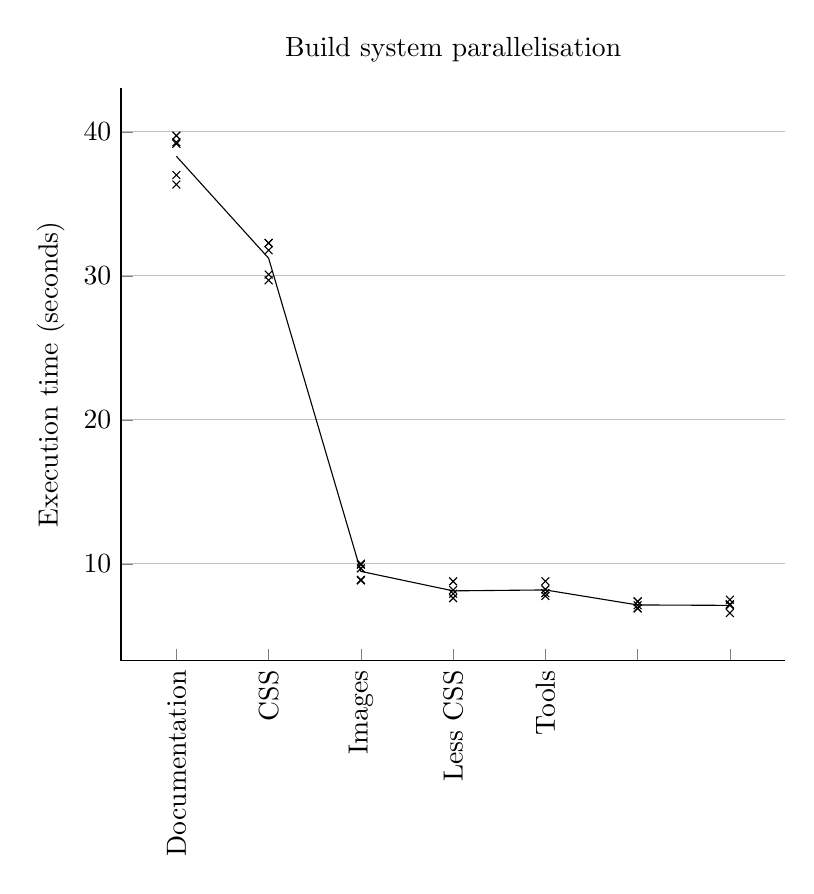
\begin{tikzpicture}
\begin{axis}[
    title={Build system parallelisation},
    axis y line*=left,
    axis x line*=bottom,
    scale only axis,
    ymajorgrids,
    xticklabels={Unmodified,
                 JavaScript,
                 Documentation,
                 CSS,
                 Images,
                 Less CSS,
                 Tools},
    x tick label style={rotate=90,anchor=east},
    ylabel={Execution time (seconds)}
  ]
% PLOT: Results
\addplot+[only marks,
          mark options={color=black},
          mark=x
]
coordinates{
  (1,39.169)
  (1,37.001)
  (1,36.344)
  (1,39.74)
  (1,39.276)
  (2,32.287)
  (2,29.689)
  (2,30.088)
  (2,31.775)
  (2,32.275)
  (3,8.887)
  (3,8.849)
  (3,9.68)
  (3,9.937)
  (3,10.007)
  (4,8.176)
  (4,8.777)
  (4,7.918)
  (4,7.614)
  (5,7.761)
  (5,8.788)
  (5,8.222)
  (5,7.96)
  (6,6.915)
  (6,6.9)
  (6,7.121)
  (6,7.38)
  (6,7.385)
  (7,6.582)
  (7,7.128)
  (7,7.192)
  (7,7.159)
  (7,7.498)
};
% PLOT: Best fit line
\addplot+[mark=none,
          color=black
]
coordinates {
  (1,38.306)
  (2,31.2228)
  (3,9.472)
  (4,8.1195)
  (5,8.18275)
  (6,7.1402)
  (7,7.1114)
};
\end{axis}
\end{tikzpicture}
\caption[Graph of build system execution times with optimisations]
        {Graph of build system execution times after each optimisation
          iteration. Each value is sequential, with the leftmost
          control value being the execution time of the unmodified
          serial build system. The tests were invoked with the command
          \texttt{time (./autogen.sh \&\& ./configure \&\& make)}.}
\label{fig:build-times}
\end{figure}

\newpage
\subsection{On-demand compilation using inotify subsystem}\label{subsec:inotify}

A common desire amongst software engineers is to reduce the feedback
loop when programming between making a modification to a source file,
recompiling the sources, and executing the compiled program. The
Autotooled build system described above provided a means for
performing automated compilation of the project sources, but it must
be manually invoked by the user, and it does not run any programs once
completed. In order to reduce the feedback cycle for pip-db, a script
was written which utilises the real time event notifications provided
by the Linux inotify subsystem \cite{love2005kernel,
  shields2010inotify}, in order to invoke the build system whenever a
dependent source file is modified. In addition, it also performs
heuristic analysis to determine which parts of the project need to be
rebuilt, and will execute a development server after rebuilding. This
greatly tightens the programmer feedback cycle, as the developer need
only save a modified file in order for the build system to recompile
the required sources and launch a new server with the changes in
place, in real time.

\subsection{Homogeneous deployment and development}\label{subsec:deployment}

One of the project risks identified in the planning stage was the risk
of complex deployment of the compiled website. This is a common
problem with web development projects, where it is necessary to take a
program developed on a local machine, and transfer it to run on a
server which often has wildly different environments and
hardware. Mitigation of this risk was achieved by combining the use of
the Autotooled build system with the use of Heroku to host the
website. Heroku\footnote{Heroku | Cloud Application Platform
  \url{https://www.heroku.com/}} is a company which offers a hosting
service whereby a repository can be uploaded and an arbitrary script
executed. This means that a build script can be executed after
uploading in order to compile all of the web sources on the server
side, ensuring that differences in the environment can be compensated
for by the build system. This simultaneously mitigates one of the key
project risks, while providing a homogeneous build system which offers
full control of the configuration of the deployment server and local
development servers.

\section{Test automation}\label{sec:test-automation}

A stated goal of the project objectives is that there should be
adequate automated test coverage of any APIs. This is achieved by
using a combination of unit tests of individual software components,
and black box testing of the entire web server using controlled
datasets.

\subsection{png: Generation of test data}\label{subsec:png}

The generation of test data is achieved using a novel application of
Markov chains for the purpose of creating plausible data from existing
datasets. A Markov chain is a system used in statistical modelling of
stochastic processes, in which the transitions between each state of a
process are modelled as a function of their probability
\cite{atwood2008markov}. When applied to a body of text, a set of
Markov chains can model the probability that a given word may follow a
preceding word. Listing~\ref{lst:markov-chain} shows a JavaScript
implementation of this text parsing, building up an array of Markov
chains (\texttt{wordTrees}), as well as recording each start and end
word for sentences.

\br{}


%%%%%%%%%%%%%%%%%%%%%%%%%%%
%% Listing: markov-chain %%
%%%%%%%%%%%%%%%%%%%%%%%%%%%
\lstset{language=JavaScript}
\begin{lstlisting}[label=lst:markov-chain,caption={%
      [Markov chain implementation]
      Markov chain implementation in JavaScript.}]
for (var i = 0; i < list.length; i++) {
  var sentence = list[i].split(' ');             // Split line into words

  startwords.push(sentence[0]);                  // Record first word
  terminals.push(sentence[sentence.length - 1]); // Record last word

  for (var j = 0; j < sentence.length - 1; j++) {
    var current = sentence[j], next = sentence[j + 1];

    if (wordTrees[current] === undefined)
      wordTrees[current] = [next];               // Create a word tree
    else
      wordTrees[current].push(next);             // Add word to tree
  }
}
\end{lstlisting}


By picking a random starting word from the set of states, it is
possible to generate a syntactically correct sentence by traversing
the states by picking a random transition from one state to the next,
based on the probability of it occurring in the training set. See
Listing~\ref{lst:markov-text-generator} for a JavaScript
implementation of a Markov text generator. This method of text
generation has applications where a seemingly plausible body of text
must be generated from an input text, and has been used largely only
for novelty purposes or for the generation of spam. The Plausible
Nonsense Generator (png) is a tool which uses a Markov text generator
to parse an input CSV training input, and generates a CSV with
psuedo-random values based on these inputs.

The Plausible Nonsense Generator proved extremely valuable for the
purposes of blackbox systems testing, where it was possible to
generate test datasets by training using PIP-DB. This provided useful
test data while mitigating the risk of exposing the confidential
PIP-DB data inadvertently while developing the prototype.

\br{}


%%%%%%%%%%%%%%%%%%%%%%%%%%%%%%%%%%%%
%% Listing: markov-text-generator %%
%%%%%%%%%%%%%%%%%%%%%%%%%%%%%%%%%%%%
\lstset{language=JavaScript}
\begin{lstlisting}[label=lst:markov-text-generator,caption={%
      [Markov text generator]
      Markov text generator implementation.}]
var next = function() {
  var word = rand(startwords); // Pick a random starting word
  var sentence = [word];       // Create a sentence array

  while (wordTrees[word] !== undefined) {
    var nextWords = wordTrees[word];

    word = rand(nextWords);
    sentence.push(word);

    if (terminals[word] !== undefined)
      break;
  }

  return sentence.join(' ');
};
\end{lstlisting}

\newpage
\subsection{Test coverage using branch analysis}\label{subsec:branch-analysis}

Unit tests are used to provide fine grained testing of individual
software components. The purpose of these tests are to ensure
correctness of code and algorithms, and operate at a lower level than
whole system black box testing. Several criteria have been proposed
for assessing the adequacy of unit tests, including an analysis of the
coverages of code branches. For a given unit, the percentage of
control transfers which are tested can be used as a metric to show
indicate how thorough the testing is \cite{zhu1997software}. If every
possible branch in a unit's program flow is tested, then it is said to
have 100\% test coverage.

In practice, achieving 100\% branch coverage with unit tests becomes
increasingly impractical with software of significant
complexity. Nested conditional logic results in an infinite set of
unique paths through a program, requiring a structured approach to
determine which paths require testing and which do not
\cite{woodward1980experience}. In pip-db, the Clojure testing
framework is used to write unit tests, and the third party library
Cloverage\footnote{Cloverage
  \url{https://github.com/lshift/cloverage}.} is used to perform
automatic branch analysis of the source
code. Figure~\ref{fig:cloverage} shows the generated report for a
given source file. The output is colour coded for each line of source
input such that green shows total test coverage, yellow indicates
partial coverage and red represents untested logic. These visual
indicators of test coverage allow for a quick review of test adequacy,
and ensure that testing efforts can be focused on critical code
sections, thus achieving the project objective of providing
comprehensive automated test coverage of the API.


%%%%%%%%%%%%%%%%%%%%%%%
%% Figure: cloverage %%
%%%%%%%%%%%%%%%%%%%%%%%
\begin{figure}[H]
\centering
    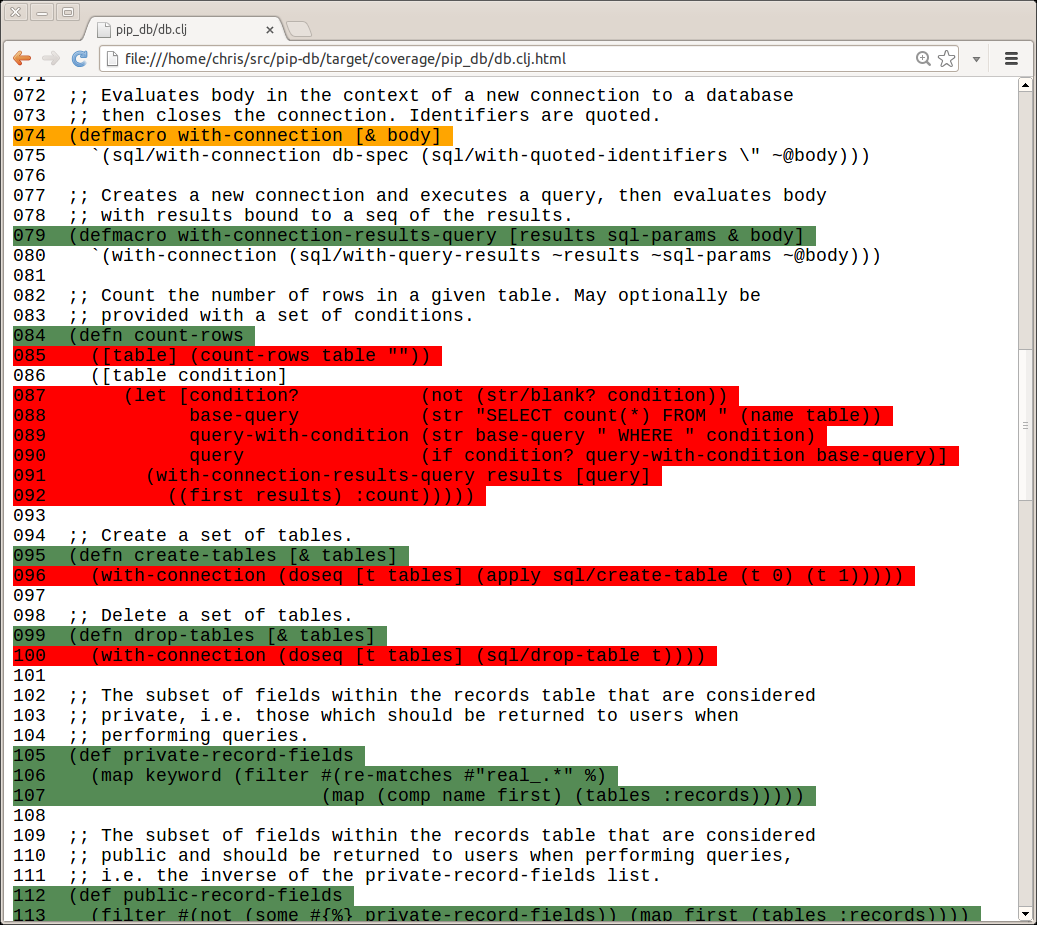
\includegraphics[width=0.82\textwidth]{assets/cloverage}
\caption[Screenshot of test coverage report]
        {Screenshot of test coverage report.}
\label{fig:cloverage}
\end{figure}


\newpage
\subsection{Continuous integration}\label{subsec:ci}

The usefulness of testing can only be asserted if tests are executed
regularly during development. This is the basic tenant of the Test
Driven Development process, which mandates that development occur in
very small cycles of continuously writing new tests concurrently with
the main development effort \cite{beck2003test}. One such technique
for encouraging test driven development is the concept of continuous
integration, in which the a cycle of development is accompanied by
continuous integration of new features into the main build, in order
to enable early regression catching \cite{fowler2006continuous,
  duvall2007continuous}. In pip-db, continuous integration testing is
provided by Travis CI\footnote{Travis CI
  \url{https://travis-ci.org/}.}, a service which uses a similar
process to Heroku as described in Section~\ref{subsec:deployment},
automatically executing the full test suite whenever a new revision is
made.

The execution of tests occurs when a revision is published, and is
performed asynchronously on a dedicated test server, which performs
the tests and reports back whether the tests passed or failed. This
way, it is possible to be continuously developing on the main project
whilst ensuring that tests are never missed. This reduces the risk of
human error causing a regression to enter into the main development
branch unnoticed, as well as reducing the development cycle by
performing testing asynchronously on dedicated hardware.

\section{Task automation}\label{sec:task-automation}

The third category of infrastructure tooling is task automation. Task
automation tools fulfil the self evident role of automating a sequence
of actions which would otherwise have to be performed manually by the
developer. The value of a task automation tool can be assessed based
on the frequency with which the task needs to be performed, and the
amount of time saved by automating it. Two examples of task automation
tools which have been written for pip-db are a dataset analysis tool
and a repository manager.

\subsection{dsa: Dataset analysis}\label{subsec:dsa}

It is important to analyse the contents of PIP-DB in order to best
understand how it should be stored and interacted with, but a manual
analysis of the dataset would taken hundreds of man hours due to its
large size. Additionally, we would need to repeat this analysis if the
dataset were to be modified. In order to mitigate the risk of a change
in the dataset during development, a dataset analysis tool (dsa) was
written which would perform automated statistical analysis of the
dataset. The dsa tool parses an input dataset and produces a machine
parsable output file containing meta data about the dataset, including
such properties as the percentages of unique values for each column, a
list of the most frequent values, the mean, range and mode of
numerical values, and a number of other properties which prove
influential in the design of the data
back-end. Figure~\ref{fig:dsa-populated} shows a graph of one of the
properties which it analyses.

The dsa tool proved valuable in the early design stages of the web
server, where a broad understanding of the dataset contents led to
justified design decisions in the back-end, with real data to support
design decisions. It also proved useful during the development of the
Plausible Nonsense Generator (Section~\ref{subsec:png}), where it
could be used to verify that the contents of generated datasets has
similar properties to PIP-DB. This reduced the time required to
prepare tests significantly.


%%%%%%%%%%%%%%%%%%%%%%%%%%%
%% Figure: dsa-populated %%
%%%%%%%%%%%%%%%%%%%%%%%%%%%
\begin{figure}[H]
\centering
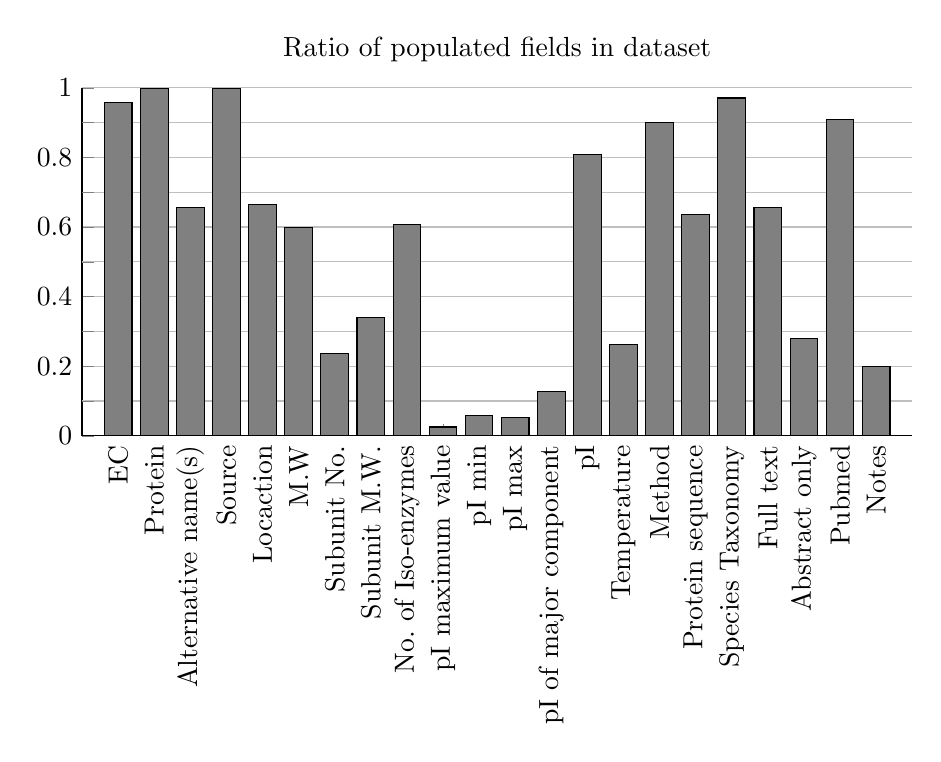
\begin{tikzpicture}
\begin{axis}[%
    title={Ratio of populated fields in dataset},
    width=\textwidth, height=6cm,
    axis y line*=left,
    axis x line*=bottom,
    ymin=0, ymax=1,
    xmin=0, xmax=23,
    extra y tick style={yticklabels={}},
    extra y ticks={0.1,0.3,0.5,0.7,0.9},
    ymajorgrids,
    x tick label style={rotate=90,anchor=east},
    xtick=data,
    xticklabels={%
      EC,
      Protein,
      Alternative name(s),
      Source,
      Locaction,
      M.W,
      Subunit No.,
      Subunit M.W.,
      No.\ of Iso-enzymes,
      pI maximum value,
      pI min,
      pI max,
      pI of major component,
      pI,
      Temperature,
      Method,
      Protein sequence,
      Species Taxonomy,
      Full text,
      Abstract only,
      Pubmed,
      Notes
    }
  ]
% PLOT: Results
\addplot+[%
  ybar,
  no marks,
  fill=gray,
  draw=black
]
plot coordinates{
  (1,0.957402597)
  (2,0.999134199)
  (3,0.656277056)
  (4,0.999307359)
  (5,0.665108225)
  (6,0.598961039)
  (7,0.237056277)
  (8,0.340952381)
  (9,0.606060606)
  (10,0.025281385)
  (11,0.057142857)
  (12,0.053333333)
  (13,0.127965368)
  (14,0.807965368)
  (15,0.262683983)
  (16,0.90025974)
  (17,0.635844156)
  (18,0.970909091)
  (19,0.656796537)
  (20,0.280692641)
  (21,0.909437229)
  (22,0.198614719)
};
\end{axis}
\end{tikzpicture}
\caption[Populated fields in dataset]
        {The proportion of populated keys for each field in the dataset.}
\label{fig:dsa-populated}
\end{figure}


\subsection{pipbot: Repository management}\label{subsec:pipbot}

The development of pipbot marks a departure from the UNIX philosophy
of creating small, single purpose programs \cite{raymond2003art}, and
instead attempts to create an all-encompassing tool for managing the
day to day activities of repository management and development. With
the sole aim of automating many of the more mundane tasks, pipbot can
be invoked as either an interactive shell or a batch mode program, and
has functionality for:

\begin{itemize}
\item \textbf{Build and deployment} Pipbot is capable of invoking the
  build system for local development, as well as deploying public
  builds to the remote web server. It can additionally generate
  reports of the current local build configuration.
\item \textbf{Generating burndowns} Pipbot can generate reports of the
  development activity over a given timespan, and since the last
  public release. This is useful for preparing for meetings by giving
  a quick high level overview of recent development efforts.
\item \textbf{Issue tracking} Pipbot interacts with the public GitHub
  API in order to be able to list, show, open and close issues. This
  removes the need to context switch between a programming editor and
  a web browser during development.
\item \textbf{Branching} Pipbot has an implementation of the branching
  model (Section~\ref{subsec:branching-model}) that allows for the
  creation and completion of feature branches. This enforces a
  consistent version control policy, making the revision history more
  uniform and informative.
\item \textbf{Release preparation} Pipbot can create release branches
  and tags.
\end{itemize}

\newpage
Implemented as a monolithic Python script, the pipbot tool was
responsible for the huge time savings throughout the course of the
project through full automation of the most common development
tasks. Figure~\ref{fig:pipbot-session} shows an example pipbot
session.

\br{}


%%%%%%%%%%%%%%%%%%%%%%%%%%%%
%% Figure: pipbot-session %%
%%%%%%%%%%%%%%%%%%%%%%%%%%%%
\begin{figure}[H]
\begin{verbatim}
$ pipbot
Hello there. My name is pipbot.
-> burndown 7 days
Comparing `master' against `master'...

  There are 56 new commits on master
  The last commit on master was 5 days, 2 hours ago
-> version
0.6.2
-> start 0.6.3
Summary of actions:
- A new branch release/0.6.3 was created, based on master.
- A new remote branch release/0.6.3 was created on origin.
- Branch release/0.6.3 tracks remote branch release/0.6.3 from origin.
- You are now on branch release/0.6.3.
- The version  number has been bumped to 0.6.3 and committed

Now, start performing release fixes. When done, use:

     pipbot finish 0.6.3

-> exit
Goodbye!
\end{verbatim}
\caption[Example pipbot session]
  {An example pipbot interactive session, in which the user begins a
   new release. User issued commands begin with the prefix
   ``\texttt{-> }''. First, the user requests a burndown of the
   repository activity over the past week; then they request the
   current version, and begin a new release with the version number
   \texttt{0.6.3}.}
\label{fig:pipbot-session}
\end{figure}
